\thispagestyle{fancy}
	
% 	\vspace{-2em} % Adjust vertical space as needed
% 	\begin{center}



% \addcontentsline{toc}{subsection}{Message of the Guest of Honour}    
% \subsection*{\textsc{Message of the Guest of Honour}}
% 	\end{center}

   
    
%     \begin{wrapfigure}{l}{0.3\textwidth}
% 		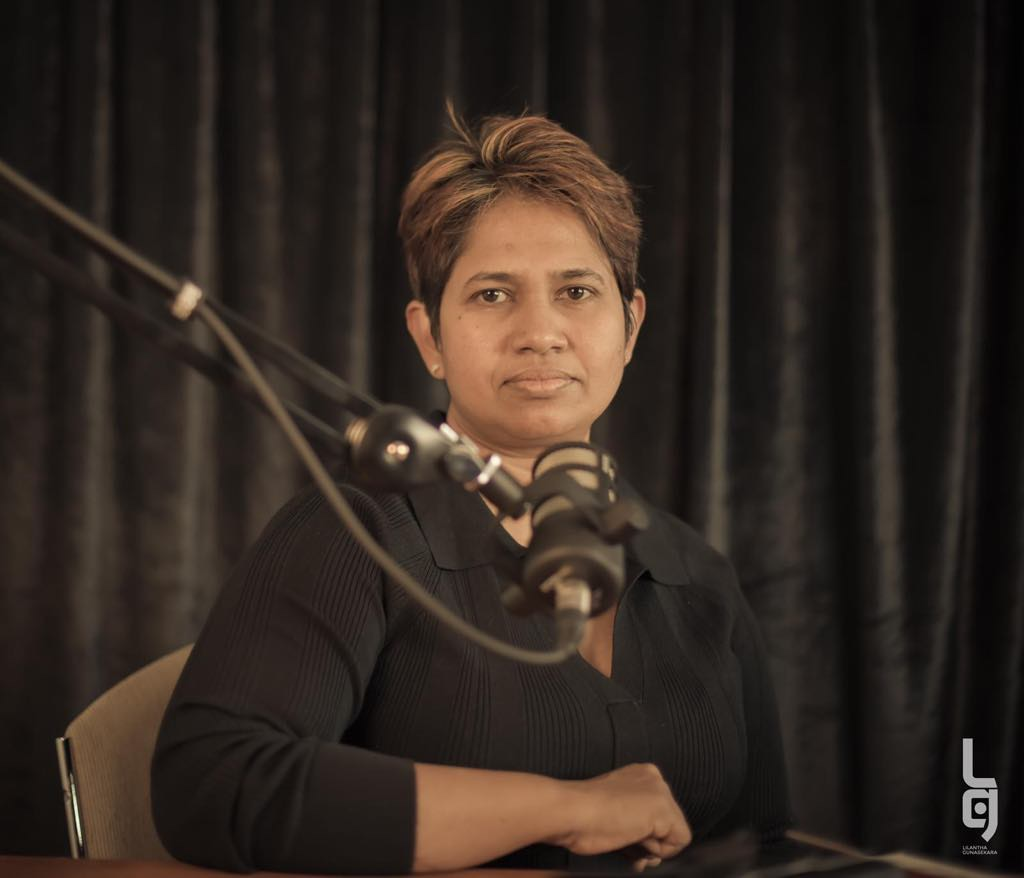
\includegraphics[width=0.3\textwidth]{Images/Guest1.jpeg}
% 	\end{wrapfigure}
% 	\vspace{2em} % Adjust vertical space as needed



\addmessage{Guest of Honour}{Guest2.jpeg}
	


It is an honor to contribute to the University of Vocational Technology Symposium 2024 as a guest speaker on the theme, “Empowering Dreams: Unlocking Higher Education Research Pathways for Vocational Excellence.”
Vocational education is a cornerstone of any nation’s economy, workforce development, and educational progress. By bridging the gap between industry needs and academic expertise, it equips individuals with skills that drive innovation and growth. Since its inception, the University of Vocational Technology has been a pioneer in this mission, nurturing talent and advancing vocational excellence in Sri Lanka.

Through its visionary free education system, Sri Lanka has the potential to achieve its aspirations by fostering research-driven solutions, enhancing global competitiveness, and shaping a resilient, skilled workforce. By investing in vocational education, we are not only empowering individuals but also driving the nation towards a future of sustainable development and economic prosperity.
The University of Vocational Technology stands as a beacon of hope and progress, demonstrating the transformative power of education. Its commitment to excellence and innovation has set a benchmark for vocational institutions worldwide. As we gather to discuss and share insights, let us remember the profound impact that vocational education has on our society. It is through these efforts that we can build a more inclusive and dynamic economy, where every individual has the opportunity to thrive.

Thank you for the privilege of sharing in this important conversation. Together, we can unlock the potential of dreams and pave the way for a brighter future. Let us continue to champion vocational education as a catalyst for national progress and global advancement.

\vspace{1cm}
	\noindent
    

Dr Nadeesha Chandrasena \\
Urban Innovator
	
	\newpage
	